\section{Przeprowadzone testy}
\subsection{Testowanie trybu normalnego}
Jako pierwsze wykonano testy trybu jednorazowo ustawiającego się nad wybranym obiektem. Aby uruchomić ten tryb, należy wpierw 
połączyć się z robotem i kamerą, wczytać wybrany model, a następnie w głównej zakładce wybrać docelowy obiekt. 
Po tym trzeba nacisnąć przycisk start i algorytm będzie zapętlony do momentu wykrycia pierwszego obiektu i wygenerowania komendy 
przesuwającej uchwyt z kamerą. 
\begin{figure}[H]
	\centering
	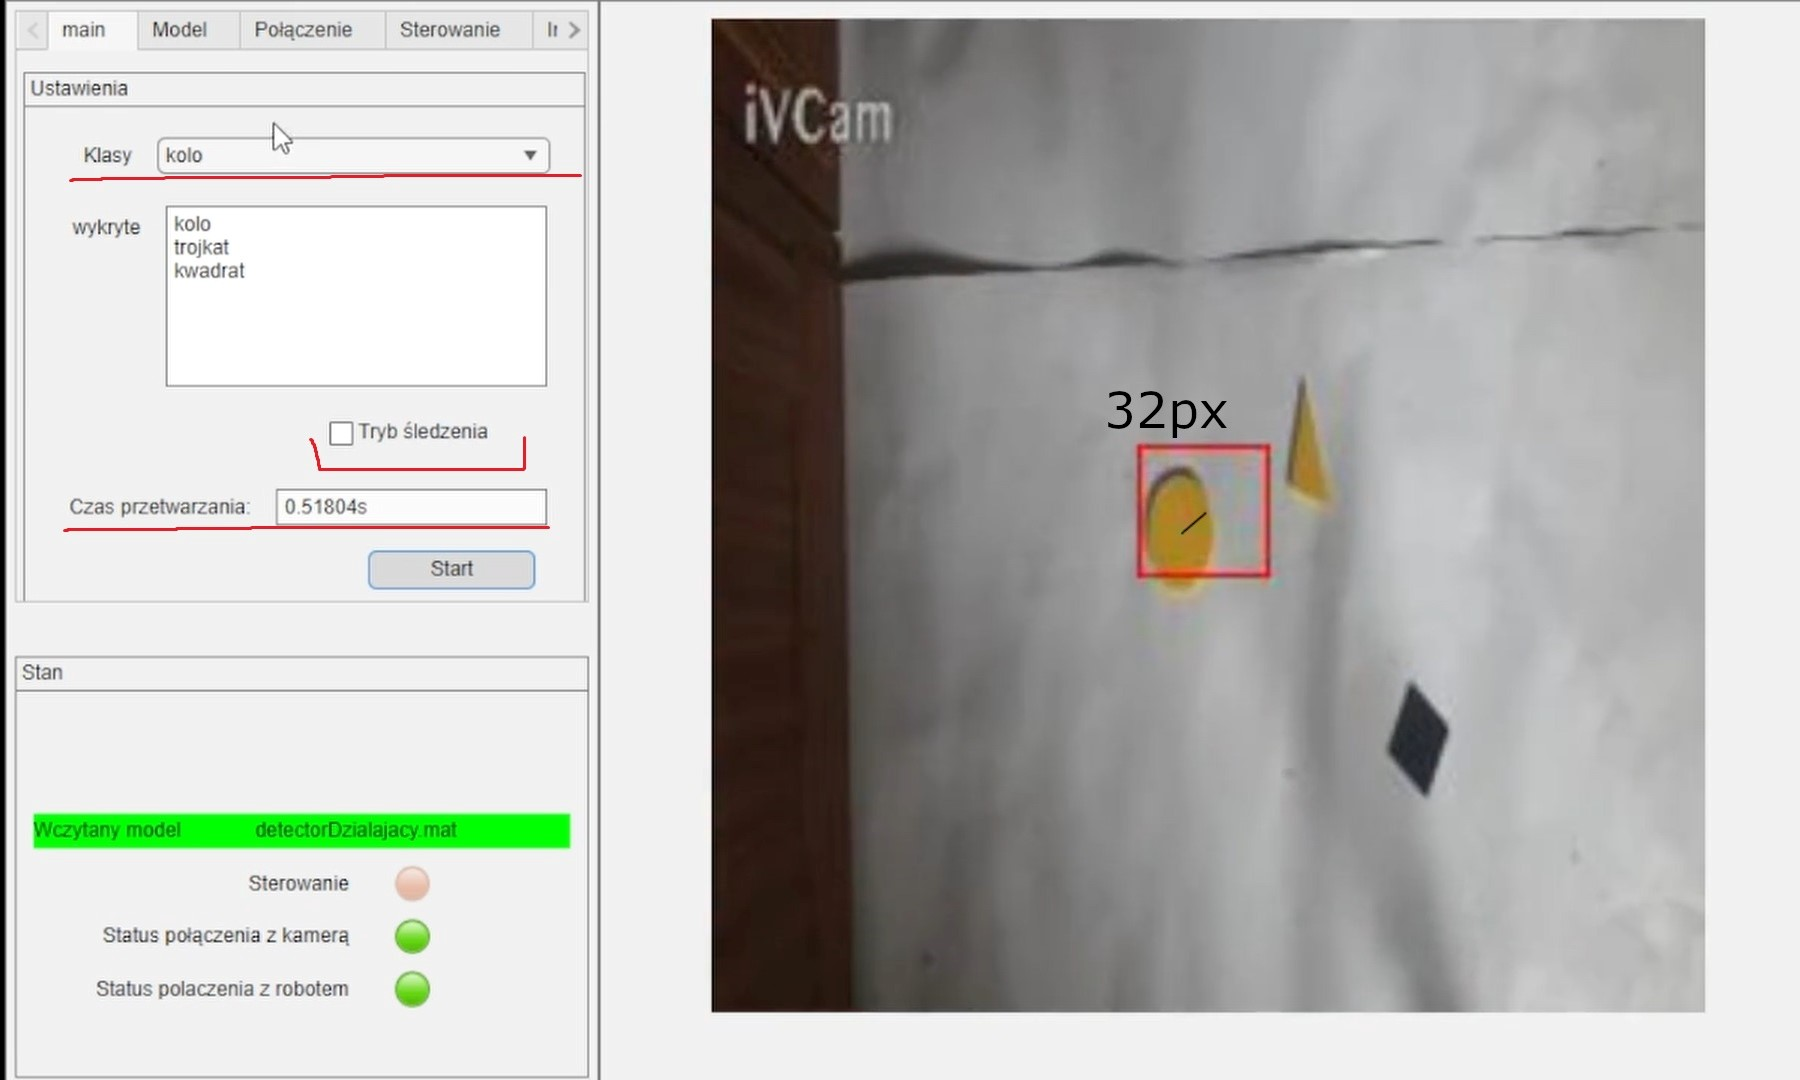
\includegraphics[width=14cm]{pages/testy/img/test1_1.jpg}
	\caption{Test trybu normalnego - wyśledzenie koła}
	\label{rys:testTrybuNormalnego1}
\end{figure}
Na rysunku \ref{rys:testTrybuNormalnego1} widać, że sieć wykryła koło a następnie wygenerowała komendę, która spowodowała przesunięcie. 
Oznaczony został element interfejsu użytkownika, pozwalający na wybranie docelowego obiektu oraz wyświetlający wszystkie znalezione na zdjęciu klasy.
W celu określenia błędu pomiędzy środkiem obrazu a osiągniętą pozycją, dodana została czarna linia. W powyższym przykładzie widać, 
że linia ta ma 32 pixele, a koło znajduję się w 'celowniku', jednak ich środki nie pokrywają się.
\begin{figure}[H]
	\centering
	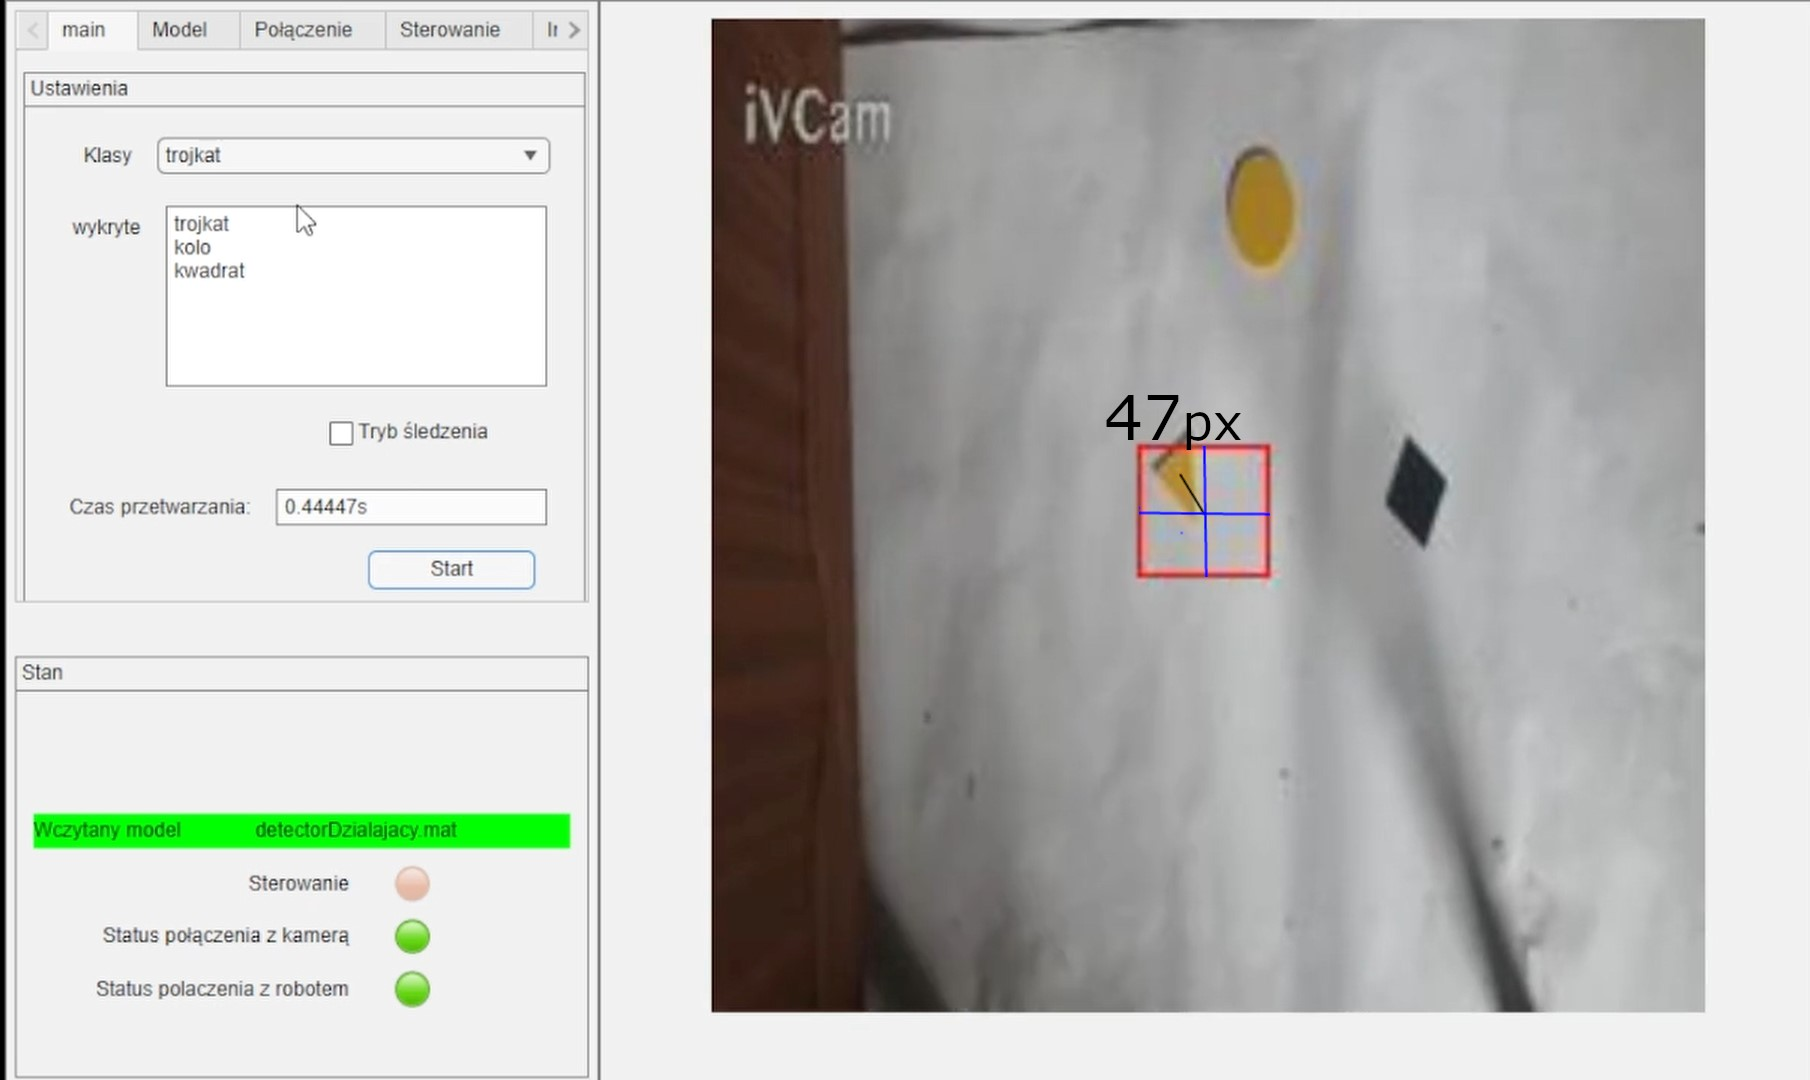
\includegraphics[width=14cm]{pages/testy/img/test1_2.jpg}
	\caption{Test trybu normalnego - znalezienie trójkąta}
\end{figure}
Przed uruchomieniem kolejnego testu, zmieniono pozycje obiektów i wybraną w programie kategorie. 
Sieć neuronowa znalazła wszystkie obiekty na obrazie, ale również w tym przypadku ostateczna pozycja cechowała się 
dużym błędem względem środków. Widać, że nawet w porównaniu do poprzedniego przypadku błąd ten wzrósł.
\begin{figure}[H]
	\centering
	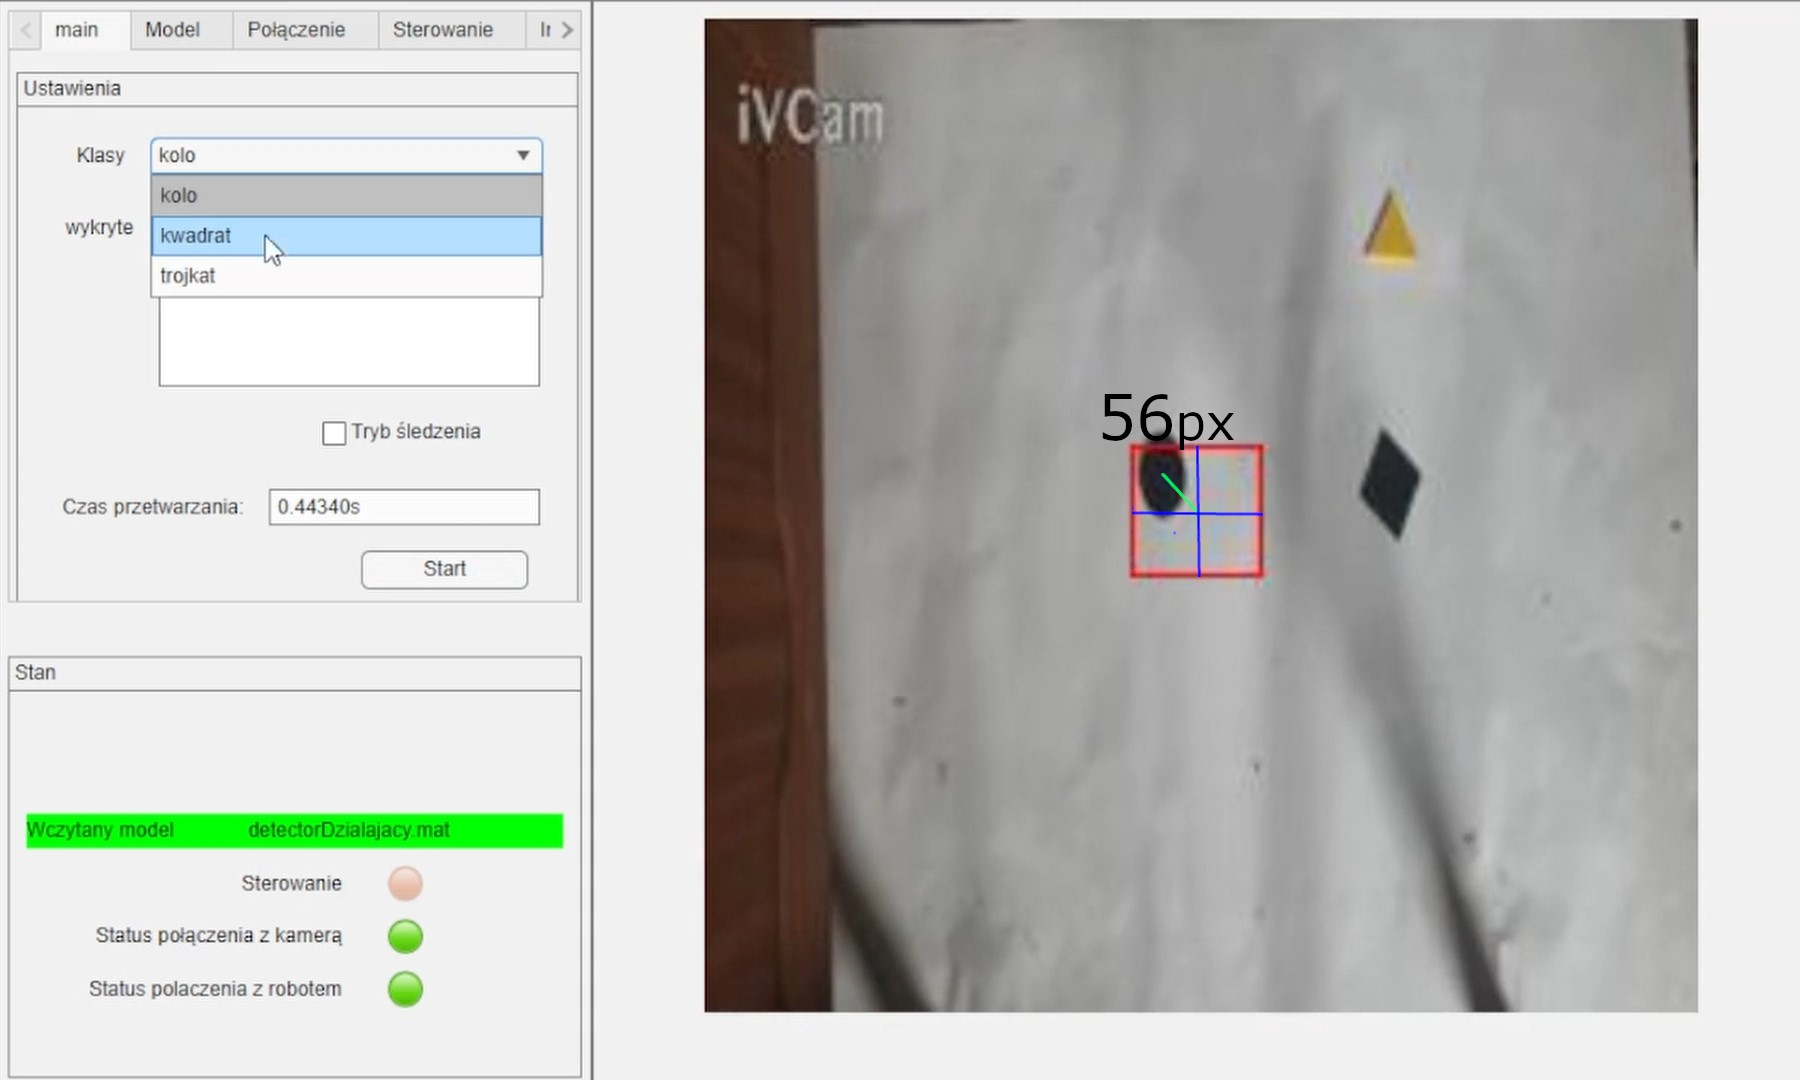
\includegraphics[width=14cm]{pages/testy/img/test1_3.jpg}
	\caption{Test trybu normalnego - znalezienie koła}
\end{figure}
Ostatni przeprowadzony test polegał na znalezieniu koła. Ponownie, jak w poprzednich przypadkach, pojawił się względnie spory błąd w wyśledzonym obiekcie. 
Analizując wszystkie te przypadki, można zauważyć, że błąd ten rośnie wraz ze zwiększeniem się odległości pomiędzy pozycją startową a końcową.
Prawdopodobnie w głównej mierze wynika to z nie dokładnie dobranego współczynników p w regulatorze wyznaczającym przesunięcie.
Warto zauważyć, że w tym trybie algorytm potrzebuje średnio około 400-500ms na analizę obrazu.
\subsection{Testy trybu śledzenia}
W związku z błędami widocznymi w poprzednim teście, opracowano drugą wersję algorytmu, który uruchomiony był w pętli 
i ciągle kompensował błędy pozycjonowania. Nazwany został śledzącym, przez to, że potrafi aktywnie śledzić dynamicznie poruszający się po scenie obiekt.
Aby uruchomić ten tryb, należy wykonać te same kroki co w poprzedniej wersji, jednak przed uruchomieniem należy zaznaczyć opcje tryb śledzenia.
\begin{figure}[H]
	\centering
	\begin{subfigure}{}
		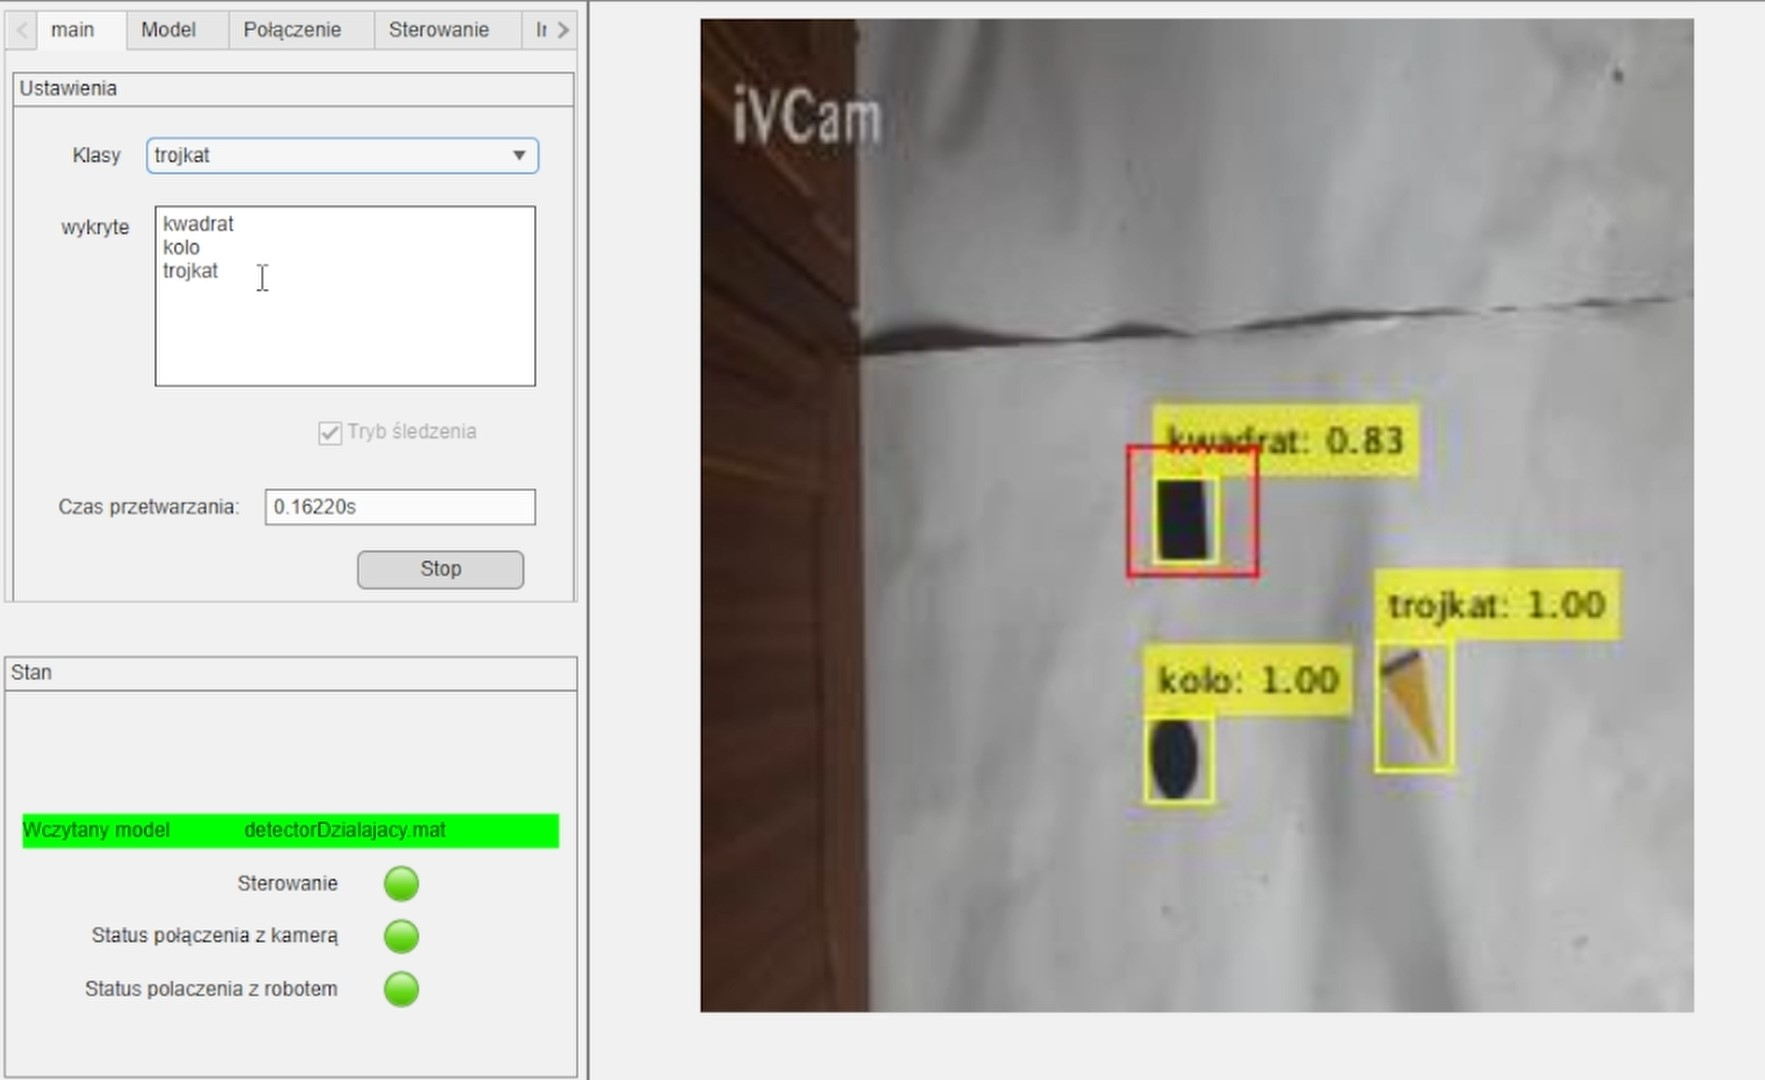
\includegraphics[width=0.5\linewidth]{pages/testy/img/test2_1_2.jpg}
	\end{subfigure}
	\begin{subfigure}{}
		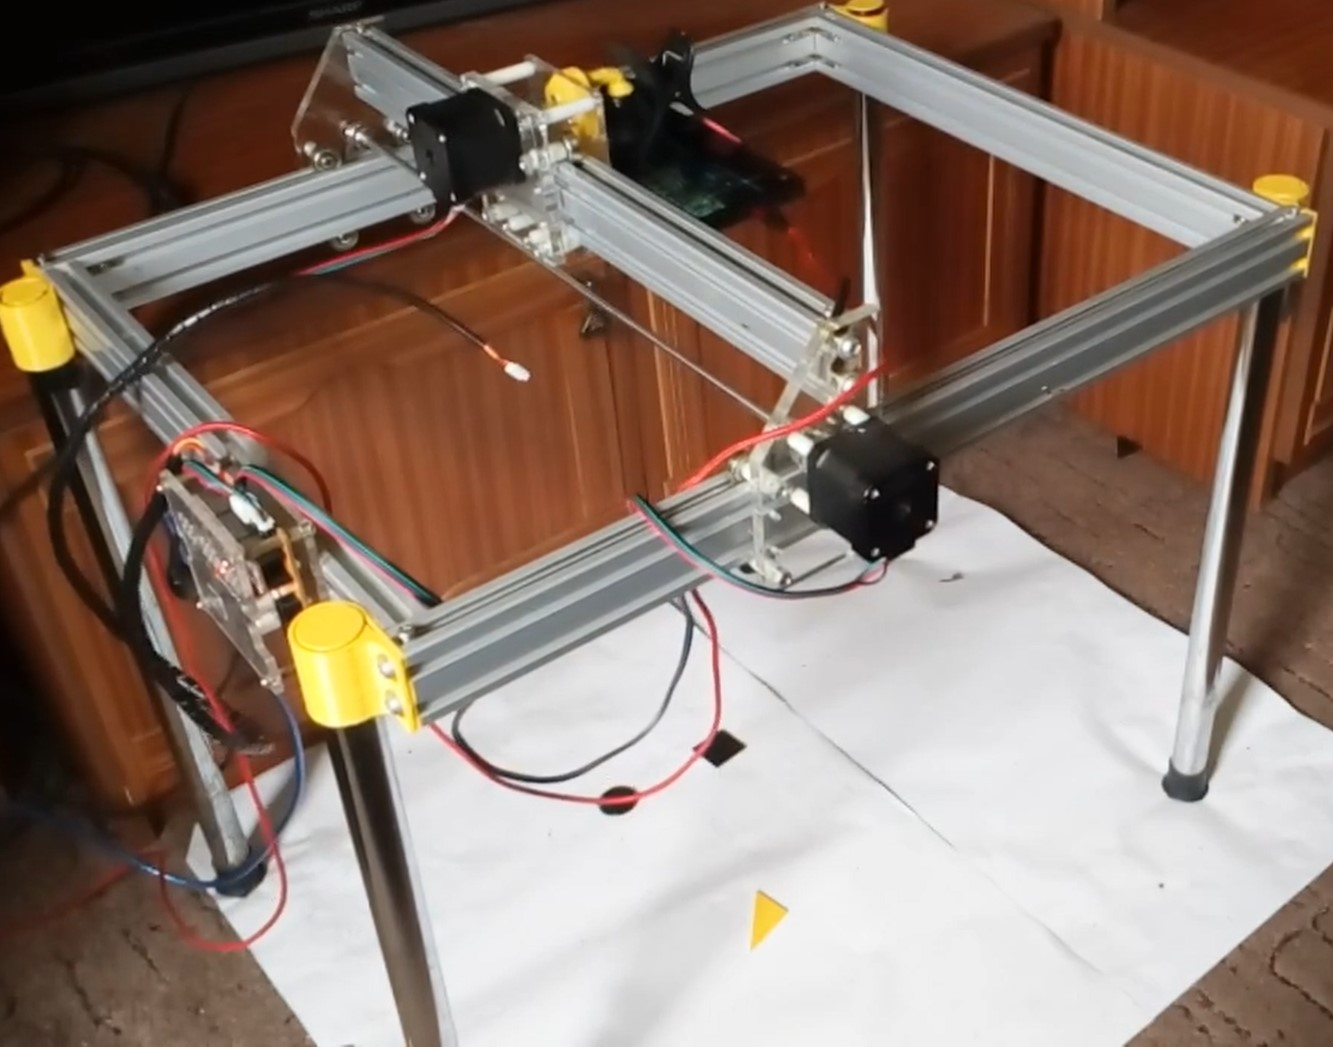
\includegraphics[width=0.4\linewidth]{pages/testy/img/test2_1_1.jpg}
	\end{subfigure}
	\caption{Tryb śledzący, widok z programu i boku robota}
\end{figure}
Jak widać w tym przypadku, sieć neuronowa analizuje każdą klatkę obrazu (widoczne są wykryte obiekty). 
Dzięki ciągłej korekcji błędów, docelowy kształt znajduje się praktycznie idealnie na środku, a po ręcznym przesunięciu
 pozycja jest automatycznie korygowana. Warto zwrócić uwagę na czas przetwarzania, który wynosi około 110ms, 
 co jest znacznie lepszym wynikiem w porównaniu do poprzedniego trybu. 
 \begin{figure}[H]
	\centering
	\begin{subfigure}{}
		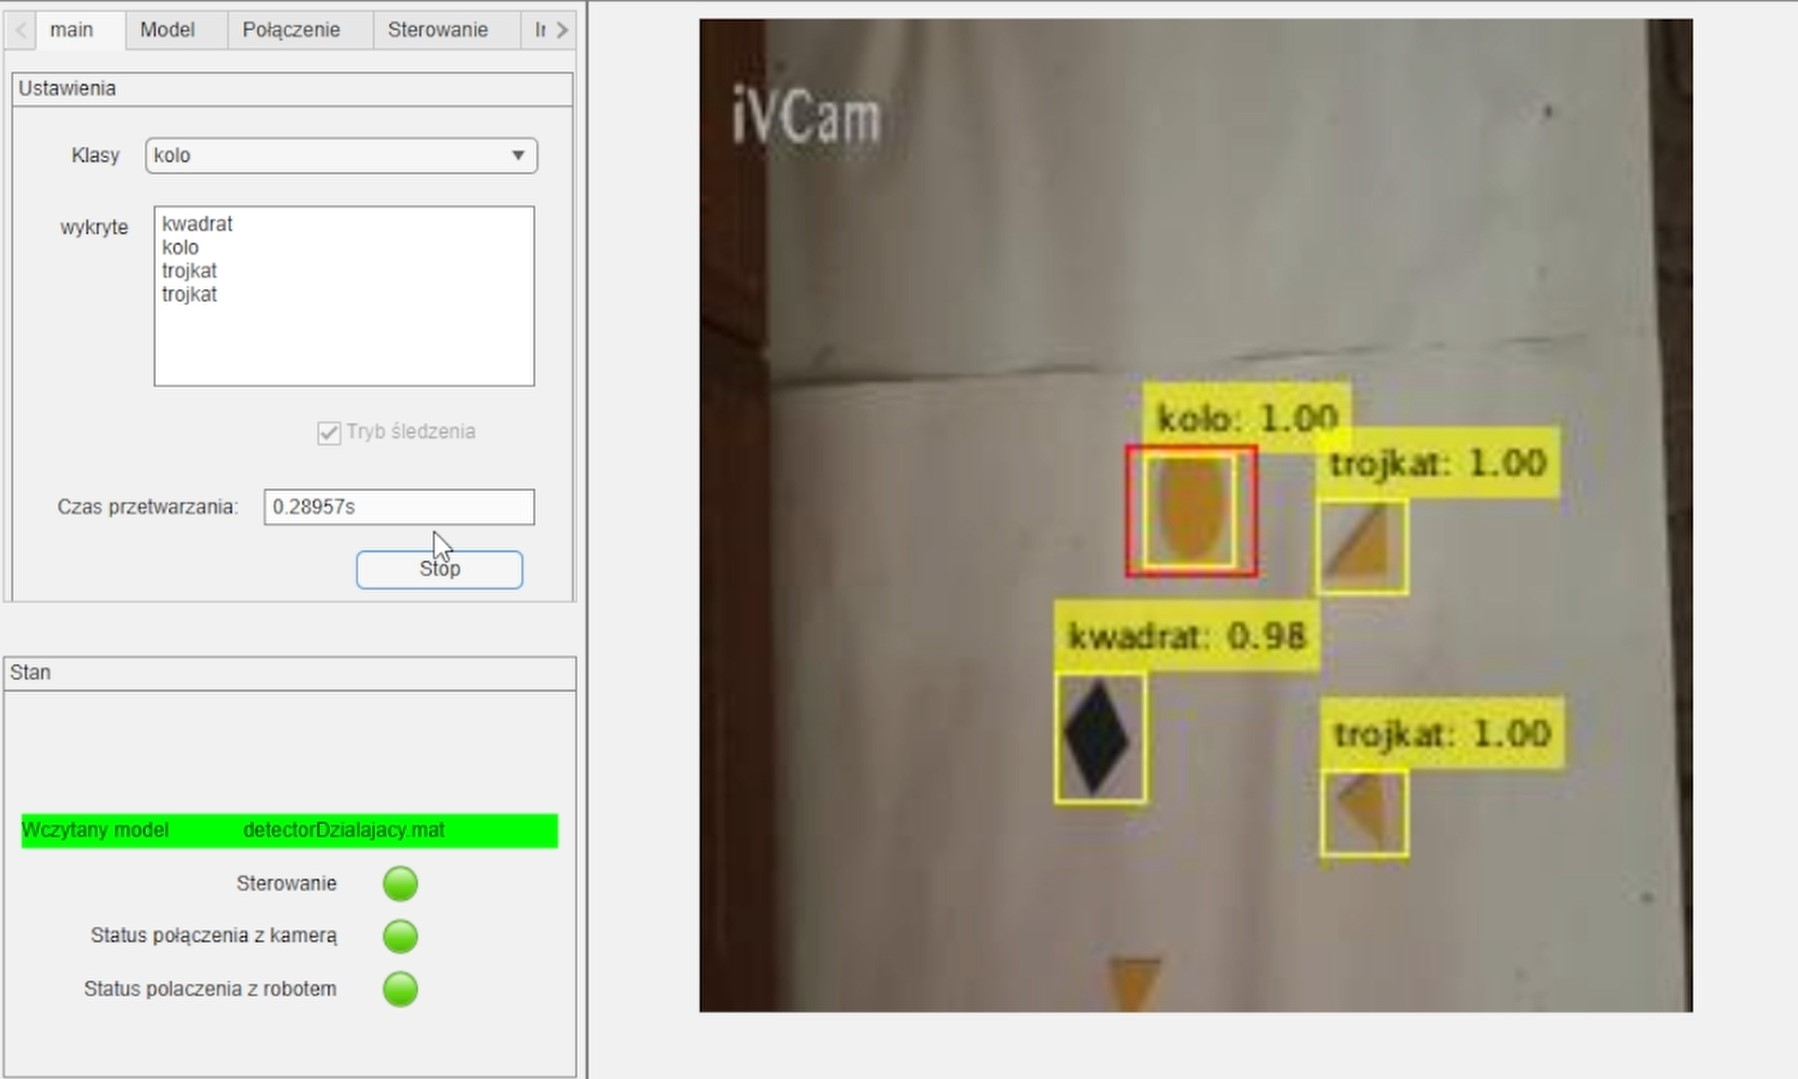
\includegraphics[width=0.5\linewidth]{pages/testy/img/test2_2_2.jpg}
	\end{subfigure}
	\begin{subfigure}{}
		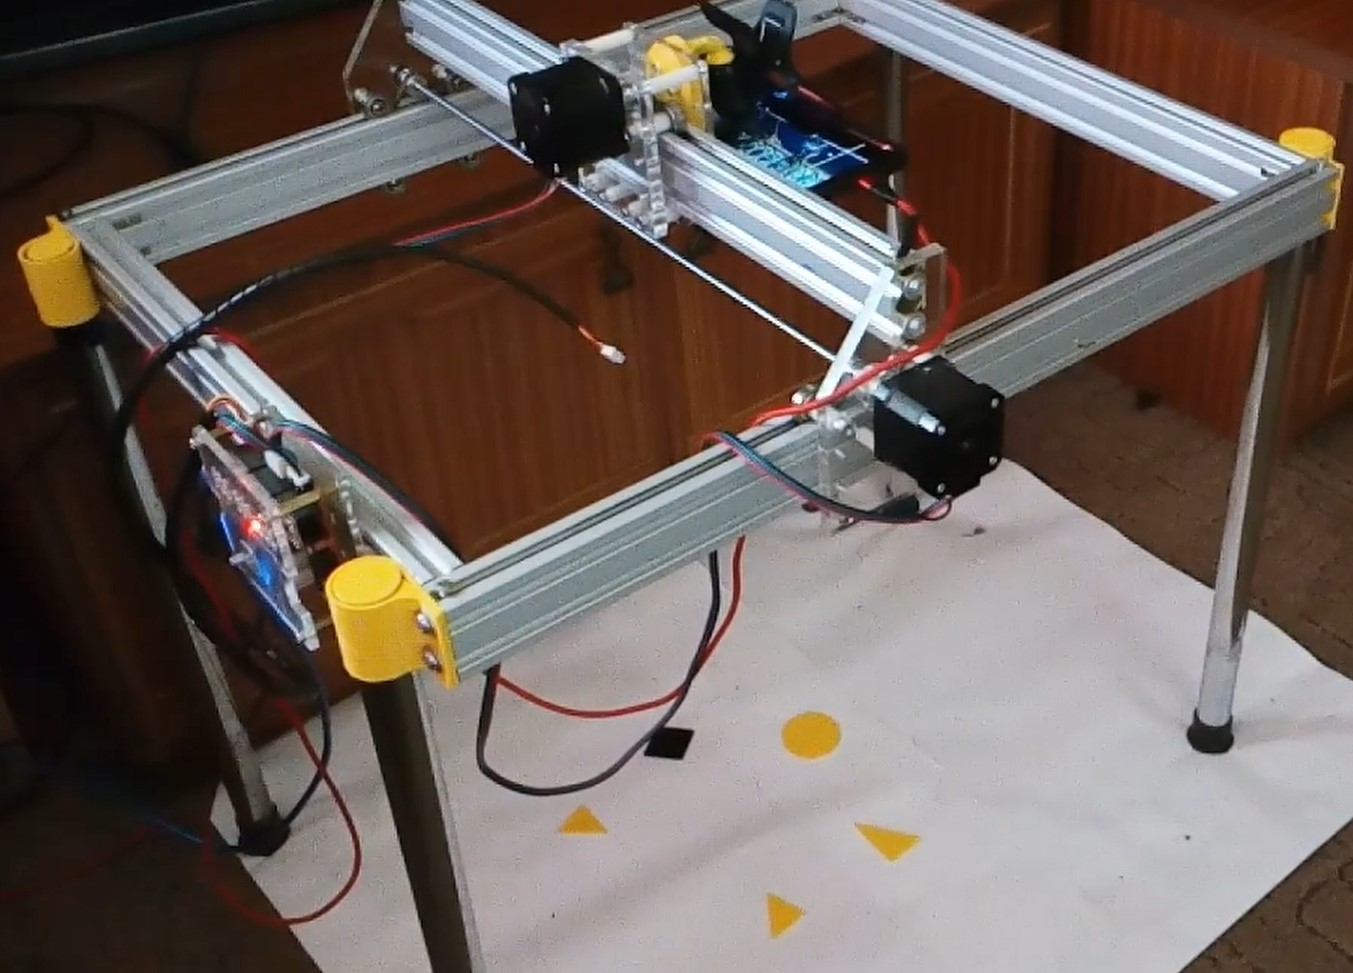
\includegraphics[width=0.4\linewidth]{pages/testy/img/test2_2_1.jpg}
	\end{subfigure}
	\caption{Śledzenie koła}
\end{figure}
Podobnie jak poprzednio, śledzenie koła działa równie dobrze, a osiągane błędy są bardzo małe. 
W porównaniu do poprzedniego trybu, w tym widoczne są duże różnice w sposobie sterowania. W pierwszej wersji algorytmu, cały ruch wykonywany był za jednym razem, a w trybie śledzenia pozycja zmieniana jest w małych krokach.